\subsection{Microservices, DevOps, Continuous Delivery and Infrastructure as Code}
\textit{This subchapter attempts to briefly explain a set of terms which will be used throughout this Master's thesis.}


\subsubsection{Microservices}
Microservices may be defined as a \textbf{cloud-native architecture} which aim is to provide software systems as a package of small services. Each of these small services should be \textbf{independently deployable} and also each of them could utilize a different technological stack and platform. The services run in separate processes and communicate with each other through mechanisms like: RESTful APIs \cite{article-micro-devops} because they utilize the language-agnostic protocol: HTTP \cite{book-pr-devops}.

Another definition of microservices is: "a microservice is simply \textbf{a self-contained service that does one thing}. If you put enough microservices together, you get an application" \cite{book-cndwk}.

Microservices are often presented as an alternative to and compared to \textbf{monoliths}. For instance, the author of "Practical DevOps" \cite{book-pr-devops} explains that, in comparison to monoliths, microservices have more integration points and suffer from a
higher possibility of failure. Furthermore, in \cite{book-cndwk} it is written that:
\begin{itemize}
\item monoliths are hard to scale, both in terms of code and also in terms of teams of people,
\item monoliths are easier to understand, because the code can be found in one place.
\end{itemize}

The schema presented in figure ~\ref{fig:microservices-vs-mono} should help to illustrate the difference between two software architecture styles.
\begin{figure}[H]
    \centering
    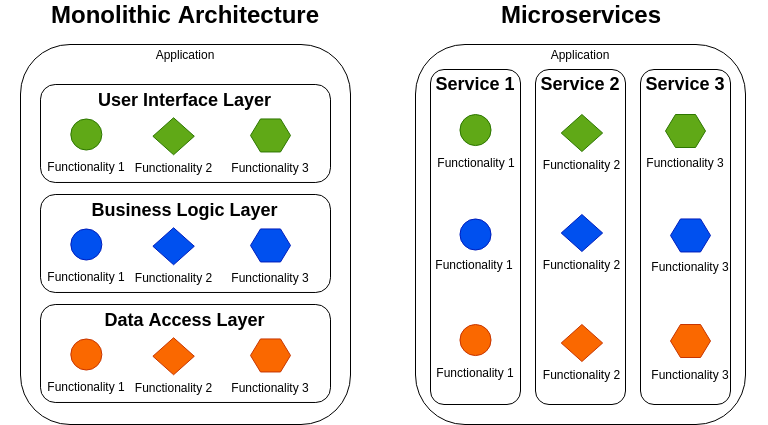
\includegraphics[width=10cm]{figures/microservices-vs-mono.png}
    \captionsetup{justification=centering,margin=2cm}
    \caption{The difference between two software architecture styles: monolith and microservices \cite{online-trans-mono-micro}}
    \label{fig:microservices-vs-mono}
\end{figure}

Microservices are not a panacea \cite{book-cndwk} and not a silver bullet \cite{article-micro-devops}, but in order to design a great software system, one should be acquainted with many solutions.

\subsubsection{DevOps}
\textbf{DevOps} and microservices have been both increasingly drawing attention since 2014, according to Google Trends. DevOps can be applied to both: monoliths and microservices, but using it for microservices promotes the importance of small teams. DevOps may be explained as a set of practices which aims \textbf{to decrease the time from the point of introducing a change to a point when the change is transferred to the production environment}. DevOps also focuses on maintaining the software quality in terms of both: code and the delivery process \cite{article-micro-devops}.

Moreover, DevOps can be defined as: "a movement to reduce barriers and friction between organizational silos - development, operations, and other stakeholders involved in planning, building, and running software". The definition continues, that even though the most visible aspect of DevOps may be technology, it is \textbf{culture, people and processes which have the most impact on flow and effectiveness} \cite{book-iac}. DevOps, as a movement, has its roots in the \textbf{Agile Manifesto}. It can be said, that DevOps obeys the first rule of the mentioned Agile Manifesto: "Individuals and interactions over processes and tools" \cite{book-pr-devops}.

In "Practical DevOps" \cite{book-pr-devops}, it is explained that DevOps spans several disciplines. Both: technical and soft skills are required to incorporate the DevOps movement. The word: \textbf{"DevOps" comes from combining: "development" and "operation"}. This already may indicate, that DevOps is a practice where collaboration between many teams matters and is encouraged.

\subsubsection{Continuous Integration and Continuous Delivery}
There are many DevOps practices: forming small teams, but also \textbf{automation and Continuous Integration (CI) and Continuous Delivery (CD)} \cite{article-micro-devops, book-pr-devops}. The first time that CI was written about was by Kent Beck in the book: "Extreme Programming Explained". CI was introduced to the world as Extreme Programming practice. The idea behind it was \textbf{to continuously --- meaning very often --- verify a source code}. CI represents a paradigm shift, because without CI, a software may be deemed broken unless somebody proves otherwise. With CI, a software is proven to work with every change added to source code \cite{book-cicd}.

There are many advantages of using CI \cite{book-cicd}:
\begin{itemize}
\item CI helps to identify the change in a source code that resulted in failing tests,
\item bugs may be caught earlier in the delivery process which is cheaper and faster when compared to fixing them in already deployed production environment,
\item delivery process is automated, thus human error is limited,
\item delivery process is automated, thus it is repeatable and easily reproducible,
\item delivery process is clearly stipulated in code,
\item CI helps different team members to communicate \cite{bachelor-ha}.
\end{itemize}

In order to incorporate the practice of Continuous Integration, a \textbf{Continuous Integration server} is needed. Examples of such a server are: Jenkins \cite{online-jenkins}, GoCD \cite{online-gocd}. The second ingredient needed is \textbf{a CI pipeline}. A CI pipeline consists of several stages which provide steps, to be performed, in order to release the software. There may be a lot more stages, for instance: the test stage can be split into many stages, each running different kind of tests (integration, functional, non-functional, acceptance, etc.) \cite{bachelor-ha, book-cicd}. The pipeline starts with a user uploading their code onto a version control system. A CI server should pick up a change and initiate the pipeline run \cite{book-pr-devops}. An example pipeline is illustrated in figure ~\ref{fig:pipeline}.

\begin{figure}[H]
    \centering
    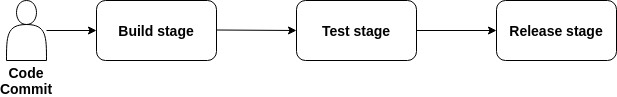
\includegraphics[width=14cm]{figures/pipeline.png}
    \captionsetup{justification=centering,margin=2cm}
    \caption{A simple example CI pipeline, consisting of a few stages, starting with a developer uploading a change of code}
    \label{fig:pipeline}
\end{figure}

Each stage of a pipeline may be either passed or failed. The failed stage indicates that some particular code change cannot satisfy the requirements of that particular stage. The stages are run in a specific order. In figure ~\ref{fig:pipeline}, the order is demonstrated with arrows. The first stage is build, then test, then release. Should the build stage fail, then neither the test nor the release stage will be run.

There exists an extension of continuous integration and it is called: \textbf{Continuous delivery (CD)}. CD verifies that a piece of software is always in a deployable state. CD is thus even more attractive than CI, because it offers even more automation \cite{online-do-cicd}.

\subsubsection{Infrastructure as Code}
Together with automation and DevOps there comes the term: \textbf{Infrastructure as Code (IaC)}. IaC may be understood as an approach to automate the infrastructure based on practices from software development. Consistent and repeatable routines are encouraged for infrastructure provisioning and configuration. There are three core practices required to implement IaC: \textbf{define everything as code} (e.g. the configuration can be saved as \textit{YAML} files), \textbf{continuously validate the code} and, \textbf{build a system from small, loosely-coupled pieces} \cite{book-iac}.

Back in time, developers dealt with software, while operations teams worked on hardware and the operating systems. Now, the hardware is in the cloud and thus, it can be handled in the same way as software. \textbf{The DevOps movement brings software development skills to operations}. It concerns both: tools and workflows \cite{book-cndwk}. The movement from deployment on-premises to the cloud also deserves a few words, but it will be handled in the subchapter: \ref{section-aws}.

\subsection{AWS - The Amazon Cloud} \label{section-aws}
\textit{This subchapter offers an introduction to cloud computing and AWS cloud and also the explanation why this particular cloud was chosen.}
\\

There are three revolutions going on \cite{book-cndwk}:
\begin{itemize}
\item the creation of the cloud,
\item the dawn of DevOps,
\item coming of containers.
\end{itemize}

These revolutions are interlinked and happen all at once. This subchapter focuses on the cloud revolution. The days of "bare-metal", before cloud, are referred to as \textbf{"Iron Age"} \cite{book-cndwk,book-iac}. The current times (after cloud was invented) are called \textbf{"Cloud Age"} and the cloud infrastructure - \textbf{Infrastructure as a Service (IaaS)}. IaaS allows to outsource not only the hardware but also the software. The outsourced software involves: operating systems, networking scripts, monitoring logic etc. \textbf{Managed services} can take care of many non-functional requirements. There is no more grand upfront investment. Having a large-scale system to build may have cost a fortune in the past. Back then, the computing power was a capital expense and now --- it is an operational one. Now, there is no fixed cost and the expense depends most often on cloud resources utilization \cite{book-cndwk, article-aws-architecting}.

\textbf{Cloud computing} may be defined as a model that provides end users with access from any device, as long as the device has an Internet access, to a shared set of cloud resources. The cloud resources involve various servers and services. Taking a step away, there may be differentiated four \textbf{deployment models}: private cloud, community cloud, public cloud, hybrid cloud. Private cloud means that the software is deployed on-premises, locally. Apart from that, there are also \textbf{service models}, which the most popular are \cite{article-poni-cloud}:
\begin{itemize}
\item Infrastructure as a Service (IaaS),
\item Platform as a Service (Paas),
\item Software as a Service (Saas).
\end{itemize}

Public clouds like: Amazon AWS, Google Cloud Platform or Microsoft Azure represent IaaS. In the Amazon whitepaper "Architecting for the Cloud" \cite{article-aws-architecting}, many \textbf{cloud computing benefits} are listed:
\begin{itemize}
\item near zero upfront infrastructure investment,
\item just-in-time infrastructure --- meaning that it is simple to scale the applications,
\item more efficient resource utilization --- resources can be reserved or required on demand (instantly),
\item usage-based costing --- users do not pay for allocated but unused infrastructure,
\item reduced time to market --- some jobs can be run parallely.
\end{itemize}

Furthermore, AWS offers \textbf{a highly reliable and scalable infrastructure} \cite{article-aws-architecting}, ensures \textbf{attractive SLAs} (e.g. AWS promises to keep a Monthly Uptime Percentage of at least 99.99\% for compute resources) \cite{online-aws-sla} and it is also \textbf{widely adopted and provides many various services} \cite{cncf-2019}. These are the reasons why AWS was chosen for this thesis. The charts in figures \ref{fig:cncf-aws-pop1} and \ref{fig:cncf-aws-pop2} present the popularity of AWS solutions.

\begin{figure}[H]
    \centering
    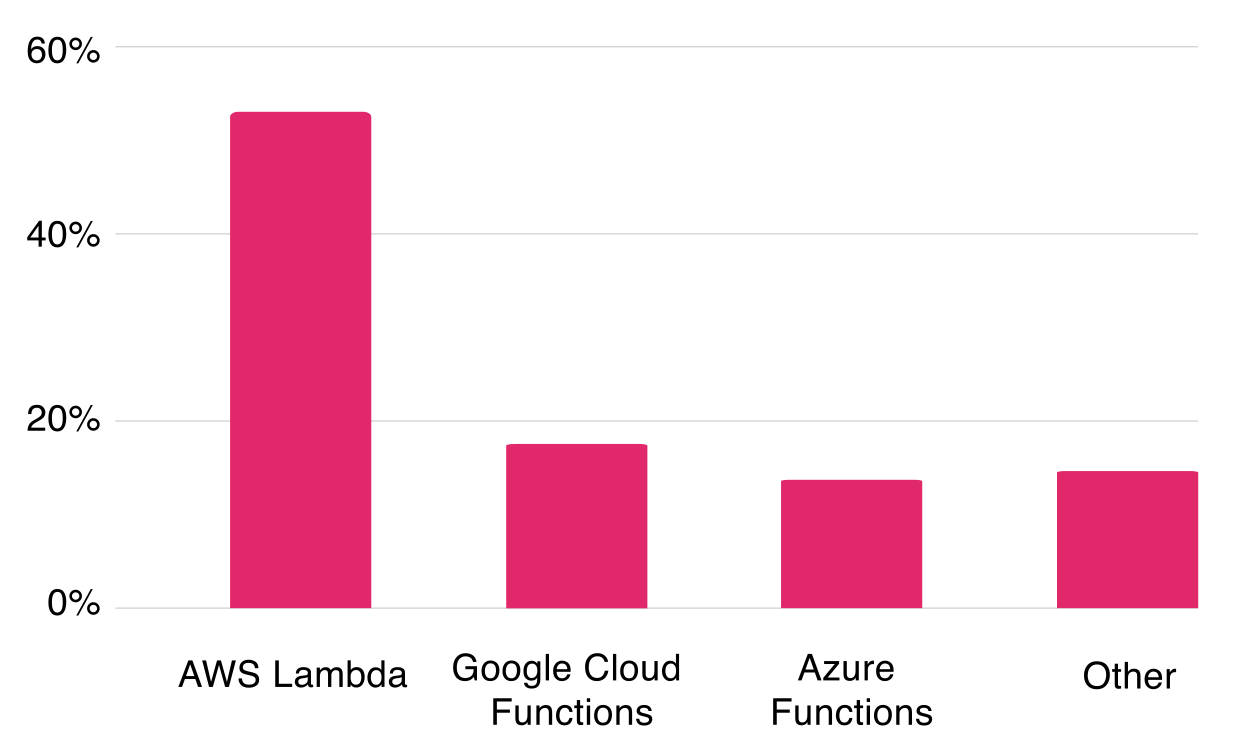
\includegraphics[width=6cm]{figures/cncf-aws-pop1.png}
    \captionsetup{justification=centering,margin=2cm}
    \caption{Hosted serverless platforms preferred by CNCF community during September and October 2019 \cite{cncf-2019}}
    \label{fig:cncf-aws-pop1}
\end{figure}
\begin{figure}[H]
    \centering
    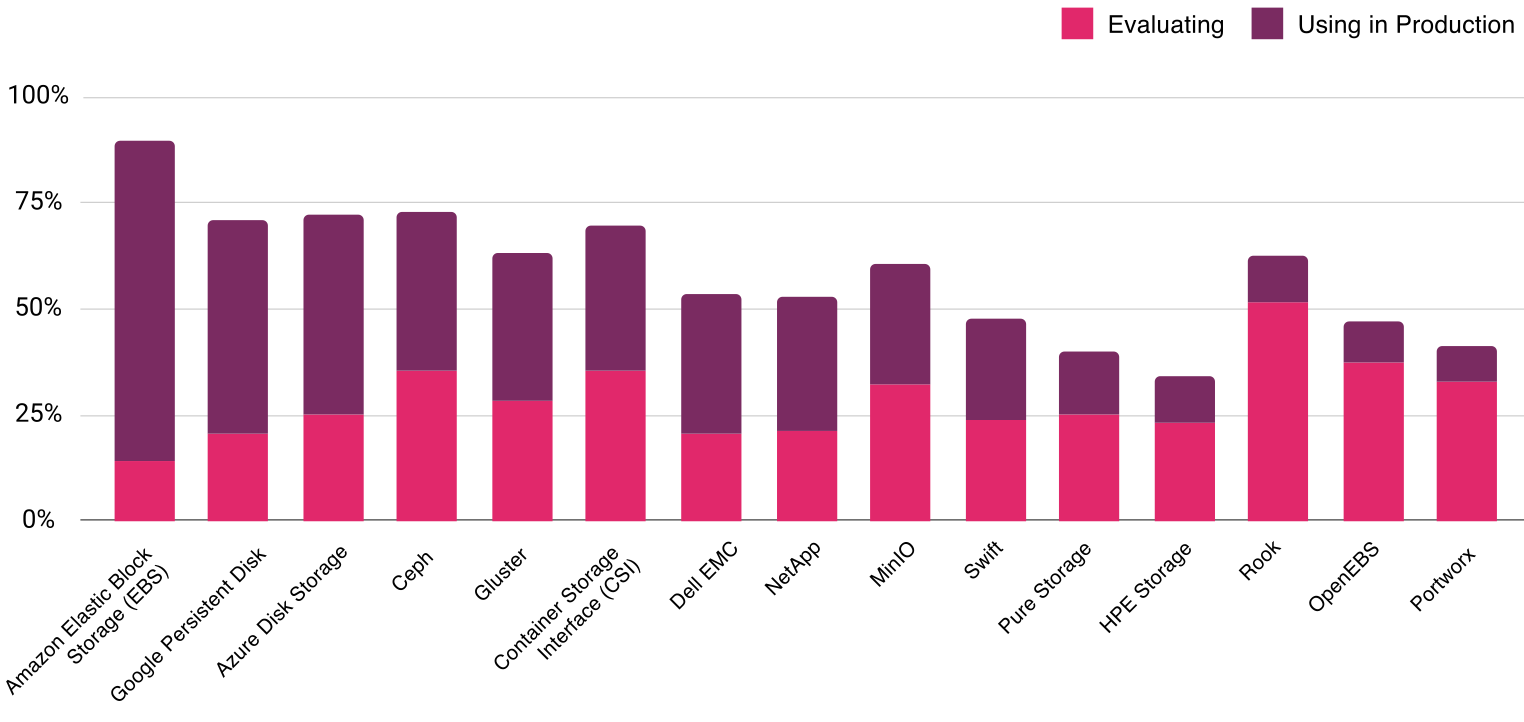
\includegraphics[width=13cm]{figures/cncf-aws-pop2.png}
    \captionsetup{justification=centering,margin=2cm}
    \caption{Cloud native storage preferred by CNCF community during September and October 2019 \cite{cncf-2019}}
    \label{fig:cncf-aws-pop2}
\end{figure}

\textbf{CNCF} is an abbreviation from \textit{Cloud Native Computing Foundation}. It is a non profit organization which fosters communities to support growth and health of cloud native open source software. CNCF adopts Cloud Native projects and catalogs them, depending on their maturity level. They also regularly conduct surveys concerning the Cloud Native and container-related technologies \cite{cncf-services}.



\subsection{Docker containers}
\textit{This subchapter provides an introduction to Docker containers and also compares them to Virtual Machines.}

In the old times, software was installed \textbf{on physical hardware directly}. Then, \textbf{virtualization and Virtual Machines (VMs)} were invented. The next great invention, after VMs, were \textbf{Docker containers}. In 2013 Docker was created as a standard way to manage containers\cite{book-devops-k8s}.

There are many advantages of using VMs and Docker containers in comparison to physical hardware. Docker containers and VMs:
\begin{itemize}
\item provide safer, isolated environment --- facilitate experiments,
\item are easier to automate, manage and replace,
\item provide reproducible environment,
\item limit "works on my machine" problem,
\item offer more security, e.g. an external user may have access only to a Docker container, not to a whole physical host,
\item have additional features, e.g. memory replication.
\end{itemize}

It is claimed, that containers may be replacing VMs. One reason for this might be that there is a significantly lower overhead in case of deploying containers compared to VMs \cite{article-modelling-performance-k8s}. Furthermore, in comparison to VMs, containers provide faster resource allocation. There are many implementation of containers, but among them, Docker is probably the most adopted \cite{article-state-machine}.

Docker uses some major Linux kernel features like: \textbf{namespaces and cgroups}. Namespaces control and limit the amount of resources a process can use, while cgroups manage the resources of a process group. They both help to provide isolation and resource limitation \cite{art-byza,book-devops-k8s}.

In order to be able to work with Docker containers, one has to know the \textbf{difference between a Docker container and a Docker image}. A Docker image is a read-only template. It has some software installed and configured. Each image has a name and a tag, which serves the same purpose as a software version. One image may be based on other image. There are many images available which are open-source and free, e.g. "debian:10.3" \cite{online-dh-debian}, "ubuntu:16.04" \cite{online-dh-ubuntu}. It is easy to build one’s own image, basing on the available images \cite{online-docker-doc}.

Below, there is an example of a source code which creates (builds) a Docker image. Just one file is enough for this task: \textbf{a Dockerfile} (listing \ref{lst:dockerfile}).

\begin{lstlisting}[basicstyle=\scriptsize,caption={A Dockerfile to build a Docker image with SSH server installed. Based on Docker official documentation \cite{online-docker-doc-bi}},captionpos=b,language=Bash,xleftmargin=0.3cm,label={lst:dockerfile}]
FROM ubuntu:16.04

RUN apt-get update && apt-get install -y openssh-server
RUN mkdir /var/run/sshd
RUN echo 'root:THEPASSWORDYOUCREATED' | chpasswd
RUN sed -i 's/PermitRootLogin prohibit-password/PermitRootLogin\
  yes/' /etc/ssh/sshd_config

# SSH login fix. Otherwise user is kicked off after login
RUN sed 's@session\s*required\s*pam_loginuid.so@session\
  optional pam_loginuid.so@g' -i /etc/pam.d/sshd

ENV NOTVISIBLE "in users profile"
RUN echo "export VISIBLE=now" >> /etc/profile

EXPOSE 22
CMD ["/usr/sbin/sshd", "-D"]
\end{lstlisting}

Docker containers are claimed to be \textbf{lightweight and portable}. Thus, containers are suitable for microservices. Since microservices are loosely-coupled, failure of one microservice should not affect other microservices of an application. This architectural style is characterized by fine granularity and therefore, it makes scaling more flexible and efficient \cite{article-k8s-as-avail}.

Docker containers are utilized by big companies like:  \textbf{Netflix or Twitter} \cite{article-nonf-twitter-netflix}. Docker is a technology described thoroughly in many literature sources and therefore there is no sense in repeating it. A curious reader is referred to read the official Docker documentation \cite{online-docker-doc}.
